\documentclass[12pt]{extarticle}
\usepackage{tempora}
\usepackage[T1, T2A]{fontenc}
\usepackage[utf8]{inputenc}
\usepackage[english, ukrainian]{babel}
\usepackage{geometry}
\usepackage{graphicx}
\usepackage{multirow}
\usepackage{multicol}
\usepackage{float}
\graphicspath{{/home/artem/Pictures}}
\geometry
{
    a4paper,
    left=30mm,
    top=15mm,
    right=20mm,
    bottom=15mm,
}

\begin{document}
\begin{titlepage}
    \begin{center}
        \textbf{\normalsize{\MakeUppercase{
            Міністерство Освіти і науки України
            Національний університет "Львівська політехніка"
        }}}

        \begin{flushright}
        \textbf{ІКНІ}\\
        Кафедра \textbf{ПЗ}
        \end{flushright}
        \vspace{15mm}

        \includegraphics[width=0.4\textwidth]{lpnu_logo.png}

        \vspace*{\fill}

        \textbf{\normalsize{\MakeUppercase{Звіт}}}
            
        До лабораторної роботи №4

        \textbf{на тему:} “Створення та керування процесами в операційній системі Linux.”

        \textbf{з дисципліни:} “Операційні системи”
            
        \vspace*{\fill}

        \begin{flushright}

            \textbf{Лектор:}\\
            старший викладач кафедри ПЗ\\
            Грицай О.Д.\\
            \vspace{12pt}

            \textbf{Виконав:}\\
            студент групи ПЗ-24\\
            Губик А. С.\\
            \vspace{12pt}

            \textbf{Прийняв:}\\
            доцент кафедри ПЗ\\
            Горечко О. М.\\
        \vspace{12pt}
        \end{flushright}

        Львів -- 2023
            
            
    \end{center}
\end{titlepage}

\textbf{Тема роботи:}Створення та керування процесами в операційній системі Linux.
\vspace{12pt}

\textbf{Мета роботи:}Ознайомитися з паралельним виконанням процесів в операційній
системі Linux, дослідити прискорення виконання завдання, через
розпаралелення на процеси. Навчитися створювати процеси в операційній
системі Linux, керувати станом та моніторити їх основні параметри.

\subsection*{Теоретичні відомості}
Створення і запуск нових процесів в операційній системі Linux має
свої особливості. Одразу після самозавантаження ядра, що відновлюється
із стиснутого стану, запускається процес ініціалізації системи init або
systemd через копіювання ядра системним викликом fork та заміною
образу створеного процесу системним викликом exec. Таким ж чином
процес ініціалізації запускає всі необхідні служби і програми, утворюючи
при цьому дерево процесів зі строгою ієрархією. Тобто всі нові процеси
будуть створенні вже існуючим процесом (в крайньому випадку процесом
init або systemd). Процес який ініціює новий процес називають
батьківським (parent), а створений процес - дочірнім (child).

Отже, якщо виконання fork() успішне, то він повертає різні значення
для батьківського і дочірнього процесу: 0 - для дочірнього та PID
дочірнього процесу для батьківського. І дочірній і батьківський процес
починають своє виконання відразу після виклику fork().
Якщо новий процес не вдалось створити, то повертається значення
-1 в батьківський процес і встановлюється значення помилки в errno. Це
може статися, якщо в системі замало ресурсів для створення нового
процесу (наприклад перевищили максимально дозволену кількість
процесів: RLIMITNPROC для getrlimit(), або бракує пам’яті), а також при
тупикових ситуаціях, що можуть виникнути у ядрі.

\subsection*{Індивідуальне завдання}

Функція: $\frac{x * x^2 * x^3}{cos x}$\\

Програми для диспетчера задач: табуляція з другого завдання, пошук чисел фібоначі

\subsection*{Хід роботи}

\paragraph{I.} Ознайомитися з системними викликами для процесів. Опрацювати
приклади з методичних рекомендацій.

\vspace{12pt}
Я ознайомився розділяти програму з виокремленням процесу на батьківський і дочірній та без нього,
що буває якщо створення процесів виходить з-під контролю, як можна дізнатись інформацію про статус дочірнього процесу.

\paragraph{IІ.}Табуляція функції
\begin{figure}[H]
    \centering
    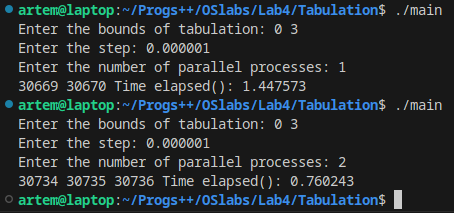
\includegraphics[width=0.90\textwidth]{tab.png}
    \caption{Tabukation}
\end{figure}

\begin{center}
    \begin{tabular}{| c | c | c | c |}
        \hline
        Діапозон &Крок& К-сть процесів & Час виконання(s)\\
        \hline
        0 - 3 &  0.1  & 1 & 0.000715 \\
        0 - 3 &  0.1  & 2 & 0.001221 \\
        \hline
        0 - 3 &  0.0001  & 1 & 0.018398 \\
        0 - 3 &  0.0001  & 2 & 0.009631 \\
        \hline
        0 - 3 &  0.001  & 1 & 0.002205 \\
        0 - 3 &  0.001  & 2 & 0.001648 \\
        \hline
        0 - 3 &  0.000001  & 1 & 1.447573 \\
        0 - 3 &  0.000001  & 2 & 0.760243 \\
        0 - 3 &  0.000001  & 6 & 0.341203 \\
        \hline
   
    \end{tabular}

    \vspace{12pt}
    Як бачимо прискорення прямопроцірційне кількості процесів, на які розпаралелена функція.

\end{center}
\break
\paragraph{IIІ.}Диспетчер задач

\begin{figure}[H]
    \centering
    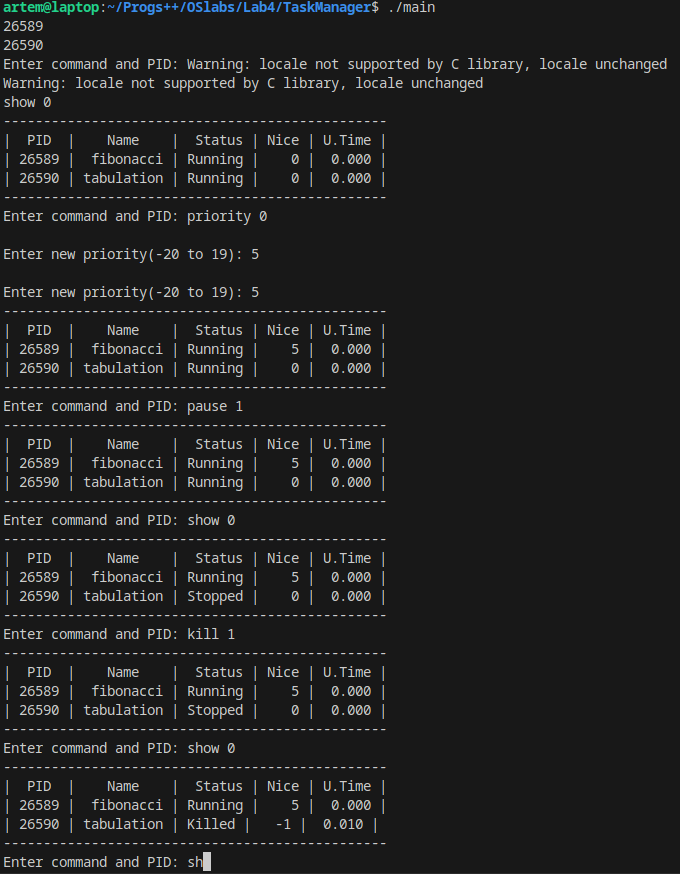
\includegraphics[width=0.90\textwidth]{task.png}
    \caption{TaskManager}
\end{figure}
\textbf{Висновок:}
Я навчився створювати процеси і отримувати про них інформацію.
 \end{document}
